% compile with pdflatex and produce svg with pdf2svg
\documentclass[tikz]{standalone}
\usetikzlibrary{arrows.meta,arrows,graphs}
\usetikzlibrary{shapes,decorations,arrows,calc,positioning,automata}
\tikzset{
  edge/.style = {
    semithick
  },
  arc/.style = {
    ->,
    semithick,
    >={[round,sep]Stealth}
  },
  bidir/.style = {
    <->,
    semithick,
    >={[round,sep]Stealth}
  }
}
\newcommand\tikzrightarrow[1][1.4em]{\tikz[baseline=-0.5ex, shorten
<=2pt, shorten >=2pt] \draw[-{Stealth[round,sep]}] (0,0) -- (#1,0);}
\newcommand\tikzleftarrow[1][1.4em]{\tikz[baseline=-0.5ex, shorten
<=2pt, shorten >=2pt] \draw[{Stealth[round,sep]}-] (0,0) -- (#1,0);}
\newcommand\tikzleftrightarrow[1][1.4em]{\tikz[baseline=-0.5ex,
  shorten  <=1pt, shorten >=1pt]
\draw[{Stealth[round,sep]}-{Stealth[round,sep]}] (0,0) -- (#1,0);}
\begin{document}
	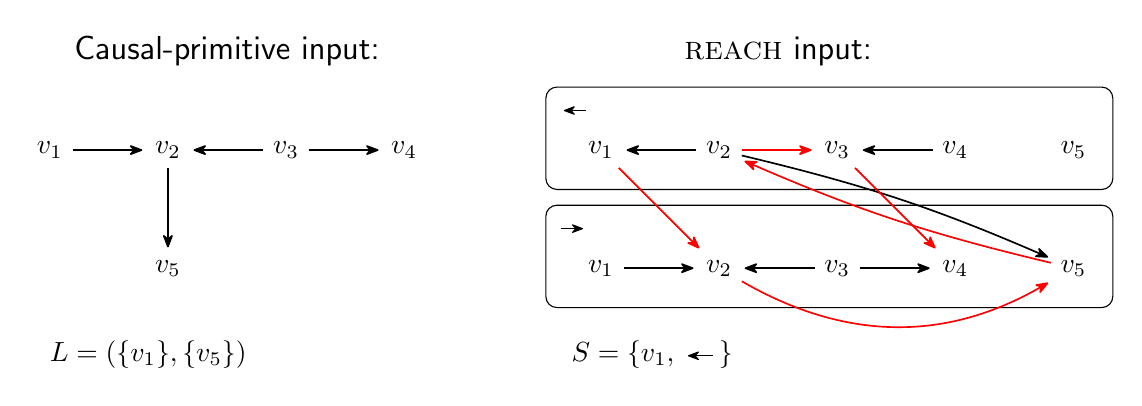
\begin{tikzpicture}
		\node (linput) at (0.75,3.0) {\textsf{\large Causal-primitive input:}};
		\node (x) at (0,1.75) {$v_2$};
		\node (m) at ($(x)+(1.5,0)$) {$v_3$};
		\node (y) at ($(x)+(3,0)$) {$v_4$};
		\node (z) at ($(x)+(-1.5,0)$)   {$v_1$};
		\node (l) at ($(x)+(0,-1.5)$)   {$v_5$};
		
		\path[arc]   (m) edge    (x);
		\path[arc]   (m) edge    (y);
		\path[arc]   (z) edge     (x);
		\path[arc]   (x) edge     (l);
		
		\node (ll) at (-0.25,-0.85) {$L = (\{v_1\}, \{v_5\})$};
%		
		\node (ltransition) at (7.75,3.0) {\textsf{\large \textsc{reach} input:}};
		\node (xu) at ($(x)+(7,0)$) {$v_2$};
		\draw [draw=black, rounded corners] ($(xu)+(-2.2,-.5)$) rectangle
		($(xu)+(5,.8)$);
		\node (mu) at ($(xu)+(1.5,0)$) {$v_3$};
		\node (yu) at ($(xu)+(3,0)$) {$v_4$};
		\node (zu) at ($(xu)+(-1.5,0)$)   {$v_1$};
		\node (lu) at ($(xu)+(4.5,-0)$)   {$v_5$};
		\node (edgestate) at ($(xu)+(-1.85,.5)$) {\small $\tikzleftarrow$};
		
		\node (xl) at (7,0.25) {$v_2$};
		\draw [draw=black, rounded corners] ($(xl)+(-2.2,-.5)$) rectangle
		($(xl)+(5,0.8)$);
		\node (ml) at ($(xl)+(1.5,0)$) {$v_3$};
		\node (yl) at ($(xl)+(3,0)$) {$v_4$};
		\node (zl) at ($(xl)+(-1.5,0)$)   {$v_1$};
		\node (ll) at ($(xl)+(4.5,0)$)   {$v_5$};
		\node (edgestate) at ($(xl)+(-1.85,.5)$) {\small $\tikzrightarrow$};
		
		\path[arc]   (xu) edge   (zu);
		\path[arc, color=red]   (xu) edge    (mu);
		\path[arc]   (yu) edge    (mu);
		
		\path[arc]   (zl) edge   (xl);
		\path[arc]   (ml) edge    (xl);
		\path[arc]   (ml) edge    (yl);
		\path[arc,bend right, color=red]   (xl) edge     (ll);
		
		
		\path[arc,bend left=5]   (xu) edge   (ll);
		\path[arc, color=red,bend left=5]   (ll) edge   (xu);
		\path[arc, color=red]   (zu) edge    (xl);
		\path[arc, color=red]   (mu) edge   (yl);
		
		\node (ll) at (6.15,-.85) {$S = \{v_1,\tikzleftarrow\}$};
	\end{tikzpicture}
\end{document}

